
\documentclass[12pt]{article}
\usepackage{amsmath}

\usepackage{indentfirst}
\usepackage[font=scriptsize]{caption}
%\usepackage[font=small]{caption}10
%\usepackage[font=footnotesize]{caption}%9
%\usepackage[font=scriptsize]{caption}%8

\usepackage[utf8]{inputenc}
\usepackage{graphicx}
\usepackage{hyperref}
\usepackage[letterpaper,margin=0.75in]{geometry}
\usepackage{setspace}
\usepackage{comment}
\usepackage{amsmath}
\usepackage{esint}
\usepackage{wrapfig}
\usepackage{lipsum}


\begin{document}

\doublespacing


\begin{center}
{\Large \textbf{Developments of a Simple Model to Elucidate the Shape of Enveloped Viruses: Motivated by Monkeypox and SARS-CoV-2}}\\[1.5ex]
{\normalsize  Hua Deng}\\

{\normalsize February 21, 2025}
\end{center}





\begin{flushleft}
\setlength{\parindent}{30pt}
\section*{Objective}
First, to develop new models and simulations to study how the viral genome architecture(its shape, length and flexibility) influences the membrane. By combining polymer physics and liquid-state physics, such as crowding effects, we hope to gain a deeper understanding of viral assembly. By simulating how viral genomes behave in confined environments, we can uncover key principles behind virus formation and stability. It could contribute to more effective strategies for prevention and treatment of viral infections, especially for viruses like Monkeypox and SARS-CoV-2.


Second, we into the pressure inside viruses helps us better understand how the virial genomes infect host cells and spread disease. When a virus packages its genetic material into its capsid/membrane, it builds up a lot of internal pressure. This pressure is key to how viruses inject their DNA or RNA into host cells quickly and efficiently. By studying this process, we can uncover new ways to block viruses from replication, such as targeting the proteins that help pack the genetic material or weakening the capsid/membrane so the virus can’t survive. It can inspire new drug delivery systems that work like viruses, help design better and more stable vaccines, and teach us more about the physical limits of DNA/RNA in extreme conditions.

%\begin{comment}
%\end{comment}
\vspace{-1em} 
\section*{Motivation}

In previous study, we developed a simple yet insightful model to investigate how monomers can self-organize into dimers, trimers, and tetramers on spherical surfaces, inspired by the trimeric spike proteins found in viruses like COVID-19. Using Monte Carlo simulations with attractive Yukawa potentials that include both radial and angular dependencies, we showed that trimers form more easily and are generally more stable than dimers. Tetramers, in contrast, require stronger attractive forces to form and are prone to aggregation when those forces become too strong. Analyses of energy and entropy contributions revealed that trimers are often more stable than dimers and, under certain conditions, as stable as tetramers. These findings are consistent with structural observations from cryo-electron microscopy studies of SARS-CoV-2 spike proteins, which show that trimers dominate the virion surface architecture\cite{Ke2020}.

\begin{figure}[!ht]
  \centering
  \includegraphics[width=0.8\textwidth,height=4cm]{spike.trimer.png}
  \caption{Left image: Simulation of the SARS-CoV-2 spike protein on a spherical surface, illustrating the progression from randomly distributed monomers (left) to trimer (center) and tetramer (right) formations. Right image: SARS-CoV-2 for Covid-19 schematic image ( CDC Public
Health Image Library) \cite{cdc-covid}}
\end{figure}


Beyond virus-related modeling, the researchers also explored how rod-like molecules
behave inside confined spaces, such as droplets or cavities, under molecular crowding. Our simulations showed that shorter rods tend to accumulate near the boundary, while longer rods align toward the center, consistent with experimental observations. These results emphasize

\begin{figure}[!ht]
  \centering
   \includegraphics[width=0.8\textwidth,height=5.5cm]{F-actin.png}
 
  \caption{\textbf{Left image:} Short DNA rods distribute near wall under molecular crowding. Long F-actin rods distribute in cavity interior and show high orientation ordering. Long F-actin rods distribute in cavity interior and show high orientation ordering.  Specific localization of 
  long DNA ($\lambda$ DNA) and F-actin in DEX-rich CAMDs.    
       \textbf{Right image:} Fluorescence microscopic images of DNA (GelGreen), actin (Alexa Fluor 546), and merged views are shown, along with polarization microscopy observations (four panels on the left). 
        The images were captured under the conditions of 120~$\mu$M $\lambda$ DNA, 10~$\mu$M actin, and 4.0~mM KCl. 
        F-actins were observed to be in a nematic liquid-crystal state at the center of DEX-rich CAMDs, while DNA molecules appeared segregated from the center. 
        In other words, long DNA strands are compressed by the aligned F-actin region, as schematically illustrated in the right panel. 
        Scale bar: 100~$\mu$m.\cite {nakatani2018}}
        %}
\end{figure}



 \noindent  the important role of both energetic and entropic factors in determining molecular organization in confined systems.


Building on this foundation, we have successfully simulated the membrane along with the spike protein on its outer surface. We are now shifting our focus from the exterior to the interior of the membrane, concentrating on the interactions between the membrane and the enclosed genome. This approach aims to provide deeper insights into how viruses are organized, how the membrane and genome influence each other’s fluctuations, and how genetic material is ultimately released—knowledge that could inform the development of new antiviral strategies.



\vspace{-1em} 

\section*{Introduction}




Viral infections have a critical impact on global health, emphasizing their role in pandemics and outbreaks. These infections pose significant risks to public health and encompass a wide range of diseases, from seasonal influenza to more severe infectious diseases such as Monkeypox and COVID-19. Both Monkeypox and COVID-19 viruses are classified as enveloped viruses, which are distinguished by their lipid membranes that surround and protect their genetic material (genomes). These membranes serve several crucial functions: they provide protection by shielding the viral genome from environmental factors and potential damage, and they facilitate transmission by enabling the virus to enter host cells. The membrane plays a key role in this process by interacting with specific receptors on host cells, thereby promoting viral infection and the delivery of the genome into the host. We need to further understand these mechanisms to develop effective prevention and treatment strategies.




Virions are acellular, meaning they are not made up of cells and therefore lack cellular components like organelles, ribosomes, or a plasma membrane. Instead, a virion consists primarily of a nucleic acid genome encased within a protein coat called a capsid. 

To elucidate the shape of enveloped viruses, one essential factor is on their genomes. The genome of a Monkeypox virus constitutes of a double stranded DNA of about 190 kb (kilo-bases) or 95 kbp (kilo-base pairs), that is 3000 nm in contour length, compared to the dimension of a virus particle at around 250 nm long\cite{erez2019diagnosis}\cite{parker2007human}. In Figure 3, the virus particles show spherical and oval shape, corresponding to immature and mature viruses, respectively.

\begin{figure}[!ht]
  \centering  
  \fbox{\includegraphics[width=0.4\textwidth,height=4cm]{electron.monkeypox.png}}
  \caption{Electron microscopic (EM) image for
Monkeypox virus particles. Oval-shaped
virus particles are mature, and spherical
particles are immature virions \cite{goldsmith2003monkeypox}}
\end{figure}







In contrast to Monkeypox viruses, SARS-CoV-2, the virus responsible for COVID-19, are spherical and their diameter is around 80-120 nm, much smaller than the size of a Monkeypox virion. In terms of
their genomes, Covid-19 viruses belong to the family of
RNA viruses as common corona flu viruses. Unlike
seasonal flu viruses, the Covid-19 virus has the longest
RNA among known corona viruses, consisting of a single
~30 kb strand of RNA with a contour length at about
1,400 nm \cite{baron2020sars}\cite{Wu2022}.

SARS-CoV-2 enters a host cell by first using its spike (S) protein to bind to a specific receptor on the surface of human cells called ACE2 (angiotensin-converting enzyme 2). This spike protein acts like a key, allowing the virus to attach tightly to the host cell. After attachment, the virus enters the cell either through direct fusion with the cell membrane or via endocytosis. Once inside, the viral envelope is removed (a process called uncoating), releasing its positive-sense single-stranded RNA genome into the host cell’s cytoplasm. This viral positive-sense single-stranded RNA acts directly as messenger RNA (mRNA) and is translated by the host's ribosomes to produce viral proteins, including more spike proteins, structural proteins, and enzymes necessary for viral replication. The viral genome is also copied to make more RNA strands. These components are then assembled into new viral particles. Finally, the new viruses are released from the cell by budding, often taking a piece of the host’s membrane with embedded spike proteins, allowing them to infect new cells. The spike protein is essential for both the entry of the virus and for determining which cells it can infect.

Viruses often have highly symmetrical structures, such as icosahedrons (20-sided shapes). This symmetry helps distribute internal evenly across the viral capsid, preventing weak spots and making the virus stable and protective of its genetic material.


When a virus infects a host, it deliberately breaks this symmetry. Doing so creates weaker areas on the surface of the capsid, which then open up to allow the virus to inject its genetic material (RNA or DNA) into the host cell. In this way, breaking symmetry is an essential part of the infection mechanism.\\




Viruses pack their genetic material DNA or RNA into capsids/membrane under extremely high pressure, often reaching tens of atmospheres, far greater than the pressure inside a champagne bottle. During the assembly of a virus, a specialized motor protein powered by ATP works to push the viral genome into the small, enclosed space of the capsid. This step requires a significant amount of energy because the DNA or RNA has to be crammed into a space much smaller than its relaxed form. As a result, the genetic material becomes tightly packed, creating considerable internal pressure. This pressure mainly arises from two factors: the repulsion between the negatively charged parts of the nucleic acid strands and the physical strain of bending a rigid, long molecule into such a confined area.\cite{BrandarizNunez2019}




This pressurization plays a crucial role in the infection process. When a virus encounters a host cell, the built-up pressure inside the capsid acts like a compressed spring, forcefully ejecting the genome into the host cell. This mechanism ensures that the viral genetic material enters the cell rapidly and efficiently, allowing the virus to take over the host’s cellular machinery almost immediately. This strategy is not limited to a single type of virus; it is conserved across many viral families, including those that infect humans, bacteria, and archaea. For instance, studies have shown that herpes simplex virus type 1 (HSV-1) can exert internal pressures of up to 20 atmospheres, which is essential for successfully delivering its DNA into the host\cite{BrandarizNunez2019}.\\




Understanding how this pressure builds up and is released is important for developing new medicines. By studying the molecular motor and the structures that hold this pressure, researchers hope to create antiviral drugs that stop the virus from ejecting its genome into the host cell. These drugs could prevent the virus from taking over the cell’s machinery and spreading, offering a new way to stop infections.



\vspace{-1em} 
\section*{Method} 
\vspace{-1em} 
\subsection*{1.1 Coase-grain models}
\vspace{-1em} 
\subsection*{Adveantage of Coase-grain model}



	Using a coarse-grain model in polymer science is really helpful because it makes things simpler and more efficient, especially when dealing with large and complex systems. One of the biggest reasons to use coarse-graining is that it saves a lot of computational power. Polymers are often made up of thousands or even millions of atoms, so simulating each individual atom takes a huge amount of time and resources. Instead of modeling each atom, a coarse-grain model groups several atoms or monomers into a "bead," which reduces the number of particles in the simulation. This allows researchers to study bigger systems and longer timescales without overwhelming their computers.

	Another advantage is that coarse-graining allows us to focus on the big picture of polymer behavior. At the atomic level, polymers have tons of detailed interactions, but often what we care about are the overall properties, like how the polymer stretches, bends, or reacts to forces. Coarse-graining simplifies this by letting researchers study these larger-scale behaviors without getting caught up in the tiny atomic details, which are often less important for understanding real-world polymer behavior.
	
	Coarse-grain models also make it easier to model interactions between polymers. Instead of focusing on each individual monomer, coarse-graining represents groups of monomers as beads. This makes the interactions between polymer chains less complex and easier to study. This is really useful for studying complicated systems like polymer networks, gels, or blends, which would be too difficult to model atom by atom.\\
	
	
	Another reason coarse-grain models are so valuable is that they help rus simulate larger systems over longer periods of time. By reducing the number of particles in the model, simulations can run much faster and allow for studies over longer timescales. Instead of simulating each tiny atom’s movement, which can take a long time, coarse-graining lets researchers study the overall behavior of the polymer chain over much longer periods. This is really useful for looking at things like polymerization processes or phase transitions that occur over time.
	
	Coarse-grain models also focuses on the important polymer properties that matter most, like flexibility, shape changes, and how polymers self-assemble. These properties are often determined by the overall structure of the polymer, not by the exact positions of every single atom. So by simplifying the model, researchers can study how polymers fold, how they form membranes, or how they interact with other molecules, without having to get into the atomic-level details.\\
	
	Finally, coarse-grain models are essential for designing new materials. When researchers are developing new types of polymers—whether for drug delivery, biodegradable plastics, or high-performance materials, these models help predict how the polymer will behave in different environments. This helps researchers optimize the materials for real-world uses without needing to simulate every tiny detail.
	In the end, coarse-grain models are incredibly useful in polymer science because they simplify complex systems, making it easier to study their behavior. They save time and computational power while still allowing scientists to focus on the big picture—like how polymers stretch, bend, and interact—helping to design better materials and understand how polymers work in the real world.
	
\vspace{-1em} 
\begin{comment}
\subsection*{Assumption of Coarse grain model}
Coarse grained models come with several assumptions that are critical for their application:\\
    1. Homogeneity:\\
    It is often assumed that the system is uniform, meaning properties do not vary significantly across space. \\
    2. Bead Representation:\\
        Each bead represents a group of atoms, assuming they behave as a single entity in terms of interactions, which may not always reflect the nuances of molecular behavior. \\
    3. Simplified Interactions:\\
        The models typically ignore specific interactions at the atomic level, such as hydrogen bonding or van der Waals forces, unless they are effective at the coarse-grained level. \\
    4. Mean-Field Approximations:\\
        Coarse-grained models often use mean-field approximations, averaging the effects of all other particles on any given particle, simplifying the interactions that can be complex in real systems. \\
    5. Fixed Connectivity:\\
        In polymer applications, it usually assumes fixed connectivity between beads, which may not fully account for the flexibility in the actual polymer chains. \\ 
\end{comment}
	
	
	
%\vspace{-1em} 

\subsection*{1.2 Monto Carlo simulation}

Monte Carlo (MC) simulation is a technique used to explore different configurations of a system by randomly sampling possible states, based on probability rules that often relate to energy. Instead of following every tiny movement of particles over time—like molecular dynamics does—Monte Carlo takes a different approach. It “jumps” from one possible state to another and decides whether to accept or reject each move depending on how favorable it is, typically using criteria like energy minimization.
This method becomes especially powerful when combined with coarse-grain (CG) models. Coarse-graining simplifies complex systems by grouping atoms or monomers into larger units, reducing the number of particles and interactions. This makes the system easier and faster to simulate, which is perfect for Monte Carlo techniques. With fewer variables to track, MC simulations can explore a much wider range of configurations in less time.
Using MC with CG models is particularly useful for studying large-scale behaviors like polymer folding, self-assembly, phase transitions, or how polymers interact with other surfaces or structures. Since you don’t need to worry about every atomic detail, you can focus on understanding the broader behavior of the material. For instance, in a coarse-grain polymer simulation, MC methods might rotate parts of the polymer chain, stretch or shift segments, or rearrange them—checking each time how these changes affect the system’s overall energy or structure.
In short, Monte Carlo simulations and coarse-grain modeling work hand in hand. Together, they make it possible to study complex polymer systems more efficiently and gain insights that would be hard to reach using more detailed, atomistic approaches.



%\vspace{-1em} 
\begin{comment}
\subsection*{Assumpations of Monto Carlo simulation}


\noindent 1. Randomness is representative
    
The simulation assumes that the random inputs it uses (often generated using pseudo-random number generators) adequately represent the variability and uncertainty of real-life scenarios.\\

\noindent 2. Independent trials
    
Each simulation run (or trial) is assumed to be independent of the others. The outcome of one run does not affect the outcome of another.

\noindent    3. Known probability distributions
    
The input variables must follow known probability distributions (e.g., normal, uniform, triangular, etc.). The accuracy of the results relies heavily on how well these distributions reflect real-world behavior.

\noindent  4. Large number of iterations
    
The law of large numbers is a key assumption — with a large enough number of trials, the average of the simulated outcomes should approximate the expected value. More iterations generally improve accuracy.

\noindent5. System/process remains stable
    
The simulation assumes that the underlying process or system doesn’t change over time during the simulation (i.e., it's stationary).

\noindent    6. Model structure is correct

The simulation is only as good as the model it's based on. It assumes the mathematical or logical structure you build reflects the real-world process correctly.




Since we use the Monte Carlo algorithm to simulate realistic physical systems, we need to ensure that our model captures the basic physical principle that two particles cannot occupy the same space simultaneously. If we do not include a repulsive potential between two beads, the simulation might generate unphysical configurations where two beads overlap—something that cannot happen in the real world. Therefore, we incorporate an excluded volume interaction (often modeled as a repulsive potential or hard-sphere constraint) to prevent such overlaps. This ensures that our simulations remain physically meaningful and reflect the correct structural and thermodynamic behavior of the system.
\end{comment}

\vspace{-1em} 
\subsection*{Excluded volume}

Excluded volume is an essential aspect of Coarse rained (CG) modeling, ensuring that two particles do not occupy the same space. Without it, particles in a simulation may overlap or penetrate each other, leading to unphysical results. To account for excluded volume, repulsive interaction potentials—such as the Lennard-Jones potential or its softer variants used in models like MARTINI or DPD—are applied. These potentials create a repulsive force that prevents particles from getting too close. Key parameters like bead size ($\sigma$) and interaction strength ($\varepsilon$) must be carefully tuned to reflect the physical size and behavior of the particles.

Before running a simulation, energy minimization and equilibration steps are typically used to eliminate any initial overlaps and ensure a stable starting configuration. Properly enforcing excluded volume is particularly important in biomolecular and polymer systems, where structural integrity and thermodynamic behavior depend on particles keeping natural distances and not overlapping unrealistically. Ignoring or mishandling excluded volume can compromise the accuracy and reliability of the simulation.





In our study of the genome–membrane system, we use a coarse-grained model and continuum model to simplify the complex biological structures and apply Monte Carlo simulation to explore their behavior. This combination allows us to efficiently capture key physical properties while significantly reducing computational cost. Monte Carlo methods also aid in fitting the parameters of the coarse-grained model, making the approach well-suited for simulating large, complex systems such as polymers and membranes with reasonable accuracy.



\vspace{-1em} 
\section*{Background} 
The genomic material of SARS-CoV-2 (single-stranded RNA) and Monkeypox (double-stranded DNA) behaves like a polymer. 

\subsection*{I. Polymer}
The polymer is a large molecule composed of identical monomers or different types of monomers linked by covalent bonds\cite {Everaers2020}. 

\begin{comment}
Both RNA and DNA are composed of long sequences of nucleotides linked together by phosphodiester bonds. 
\end{comment}

\begin{figure}[!ht]
  \centering
  
  \fbox{\includegraphics[width=0.25\textwidth,height=2.5cm]{polymer.png}}
  \caption{Polymer}
\end{figure}


Back in the 1960s and '70s, long before computational biology became mainstream, polymer scientists were already developing clever ways to simplify and understand how long-chain molecules behave. They built theoretical models like the freely-jointed chain, worm-like chain, and Gaussian chain—each designed to capture how flexible or stiff a polymer might be, and how it moves in space. These early ideas laid the foundation for what we now call coarse-grained simulations.

Around the same time, the bead-spring model, a type of coarse-grained representation, emerged—a simple yet powerful way to represent a polymer as a series of connected beads linked by springs. It proved highly effective for studying how polymers move, tangle, and interact in bulk materials, and remarkably, this basic idea is still widely used today in modern polymer simulations \cite{Kremer1990}.

Polymers are often described as long, flexible chains whose properties scale with their size. The bead-spring model captures key features such as bonding and excluded volume. However, to understand the detailed behavior of specific polymers, their chemical composition must be considered. While molecular dynamics simulations can offer a high degree of realism, they are computationally demanding and often impractical for simulating the slow dynamics of large systems over long timescales. To overcome this, more efficient coarse-grained (CG) models have been developed to strike a balance between accuracy and computational cost.

\begin{figure}[!ht]
  \centering
  \fbox{\includegraphics[width=0.75\textwidth,height=5cm]{discrete.png} }
  \caption{Different computational methods developed to study cellular membranes are valid in different length and time scales.\cite{chabanon2017systems}}
\end{figure}


\vspace{-1em} 



\subsection*{II. Membrane/Phospholipids}
Phospholipids are the main ingredients of cell and viral membranes, and their structure is actually a lot like a simple polymer. The head is connected to the tails through a small backbone, so the whole molecule looks kind of like a matchstick or a two-tailed kite. Because one part of the molecule wants to be near water and the other part wants to avoid it, phospholipids naturally arrange themselves into layers when they’re in water. These layers form flexible membranes that act a lot like soft polymer sheets—they can bend, move, and even stretch a little. In fact, scientists often use ideas from polymer physics to study how these membranes behave, especially when trying to understand things like how viruses wrap themselves up or how they enter cells.
\begin{figure}[!ht]
  \centering
  \fbox{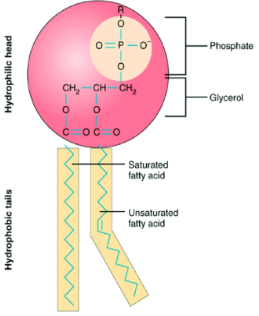
\includegraphics[width=0.45\textwidth,height=6cm]{membrane.png}}
  \caption{membrane subunit}
\end{figure}



Membranes share several important similarities with polymers that make them comparable in some ways. Both are soft, flexible materials capable of bending, stretching, and fluctuating, which reflects their shared physical nature as entropic, deformable systems. Like polymers, membranes are composed of repeating units—in this case, lipid molecules arranged in a bilayer rather than monomers linked in a chain—giving rise to a collective, cohesive structure. Additionally, membranes exhibit entropic elasticity, meaning they resist stretching and bending because such deformations reduce the number of accessible configurations, similar to how polymers respond to mechanical forces.


Despite their similarities, membranes and polymers also exhibit significant differences. A key distinction lies in their dimensionality: a polymer is typically a long, 1-D chain of monomers, while a membrane is a 2-D sheet of molecules organized in a bilayer structure. This bilayer arrangement features a hydrophobic core formed by lipid tails, sandwiched between hydrophilic surfaces of lipid head groups, giving membranes a unique amphiphilic character essential for their stability and biological function. Moreover, membranes serve a fundamentally different purpose than polymers; while polymers can form single chains that fold into complex three-dimensional structures (such as proteins), membranes create continuous, self-sealing barriers that separate and compartmentalize cellular contents, supporting life’s essential processes.


Given these differences, especially the two-dimensional fluid nature of membranes and their role in large-scale processes, a continuum model becomes especially valuable for studying membranes. A continuum model is not exactly an extension of a coarse-grained model, but rather a higher-level, more abstract description of the same system (See Figure 5). While coarse-grained models can still capture important molecular details, they often become computationally intensive or overly complex when studying large-scale, collective phenomena. In contrast, continuum models are particularly useful for exploring the large-scale, collective mechanical properties of membranes, including bending rigidity, surface tension, area compressibility, spontaneous curvature, Gaussian modulus, and, in some cases, shear elasticity. These properties describe how membranes deform, flow, and undergo shape transitions — all of which are critical for understanding their biological functions and large-scale dynamics.





\vspace{-1em} 
\subsection*{III. Genome/DNA/RNA}
DNA and RNA are long chains made up of smaller units called nucleotides. Each nucleotide is like a puzzle piece, made of a sugar, a phosphate group, and a nitrogen base. In DNA, the sugar is called deoxyribose, and in RNA, it’s ribose. The bases are the parts that carry genetic 

\begin{figure}[!ht]
  \centering
  
   \fbox{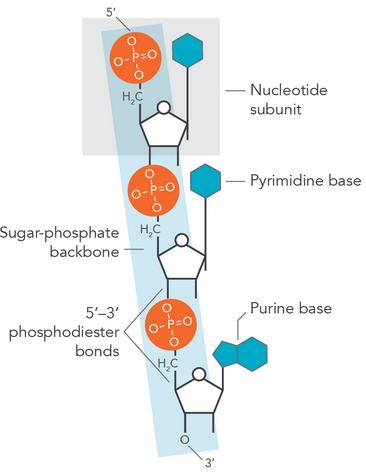
\includegraphics[width=0.35\textwidth,height=8cm]{genome.png}}

  \caption{Nucletide subunits}
\end{figure}


\noindent information—A, T, G, and C in DNA, and A, U, G, and C in RNA (with U replacing T in RNA). These nucleotides link together through bonds between the phosphate of one and the sugar of the next, forming a backbone, kind of like beads on a string. 



DNA and RNA are made of repeating units called nucleotides, similar to how polymers are made from repeating monomers. These long chains of nucleotides form biopolymers that can bend, twist, coil, and stretch like plastic or rubber polymers. This flexible structure allows DNA and RNA to fold into different shapes and form secondary structures.

Their shape and behavior depend on the nucleotide sequence, chemical interactions, and environmental conditions. They also interact with proteins, which is important for processes like gene expression and viral assembly. Because of these polymer-like properties, scientists often use polymer models to study and simulate how DNA and RNA behave










\begin{figure}[!ht]
  \centering
   \fbox{\includegraphics[width=0.45\textwidth,height=4cm]{chromatin.png}}
  
  %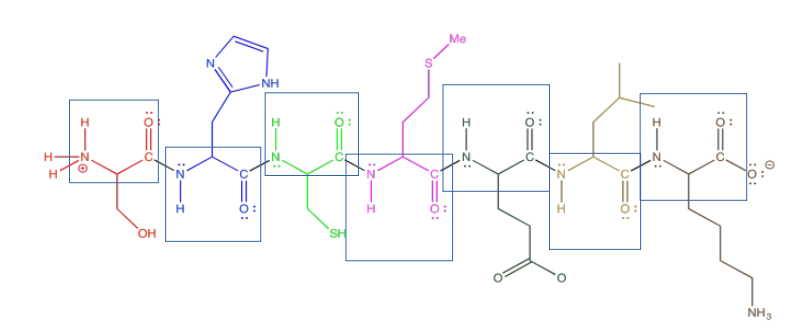
\includegraphics[width=0.3\textwidth,height=4cm]{protein.png}  % Adjust width or height as needed
  \caption{DNA, Chromatin and Chromosome\cite{byjus_chromatin}}
\end{figure}



\vspace{-2em} 
\subsection*{IV. Protein/Amino Acid chain}
Proteins are natural polymers made up of amino acids, which are like the individual links in a chain. Each amino acid has the same basic structure: a central carbon atom (called the alpha carbon) bonded to a hydrogen, an amino group (–NH$_2$), a carboxyl group (–COOH), and a unique side chain, known as the R group. These amino acids connect through peptide bonds, forming a 

\begin{figure}[!ht]
  \centering
   \fbox{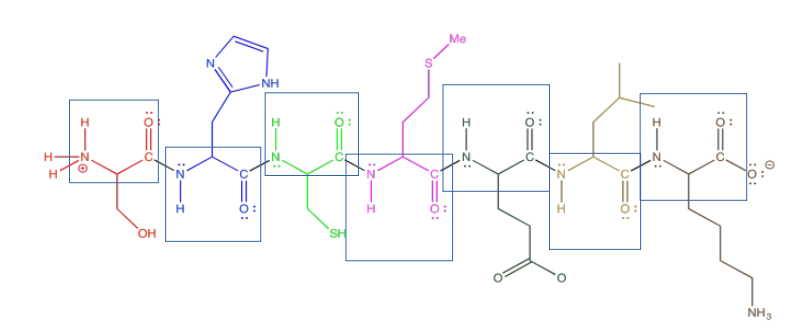
\includegraphics[width=0.5\textwidth,height=4cm]{protein.png}}
  
  %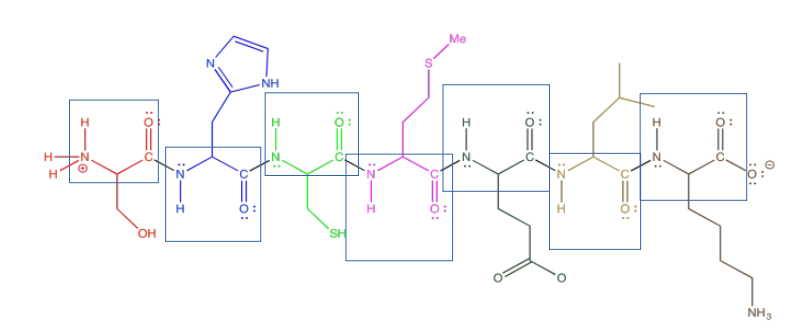
\includegraphics[width=0.5\textwidth,height=4cm]{protein.png}  % Adjust width or height as needed
  \caption{Amino acid chain}
\end{figure}

A protein is fundamentally a polymer—a long chain of amino acids linked together. In its unfolded state, this chain behaves like a typical polymer: flexible, disordered, and dynamic. As it folds, however, it transforms into a highly organized and functional structure. The folding process begins with the formation of local secondary structures, such as alpha helices and beta sheets, followed by the overall folding of the chain into a specific three-dimensional shape (tertiary structure). In some cases, multiple folded chains assemble into a larger complex, forming a quaternary structure. Despite this transformation, the polymer backbone remains; it’s simply arranged in a compact and functional form.

Once folded, a protein may not resemble a simple polymer visually or functionally. Though still composed of repeating amino acid units, these units are now intricately arranged—spiraling into helices, flattening into sheets, and looping into turns that define the protein's function. It no longer appears as a linear chain, but it retains key polymer-like properties: flexibility, responsiveness, and dynamic movement in response to its environment.

This underlying polymer nature is why coarse-grained (CG) modeling remains effective, even for folded proteins. Rather than representing every atom, CG models group atoms into larger units or “beads,” allowing us to study large-scale behaviors—such as folding, conformational changes, or molecular interactions—without the computational cost of atomic detail. Because proteins are still polymers at their core, coarse-graining offers a powerful way to explore their structure and function at a broader scale.


\begin{figure}[!ht]
  \centering
   \fbox{\includegraphics[width=0.5\textwidth,height=6cm]{complex.protein.png}}
  
  %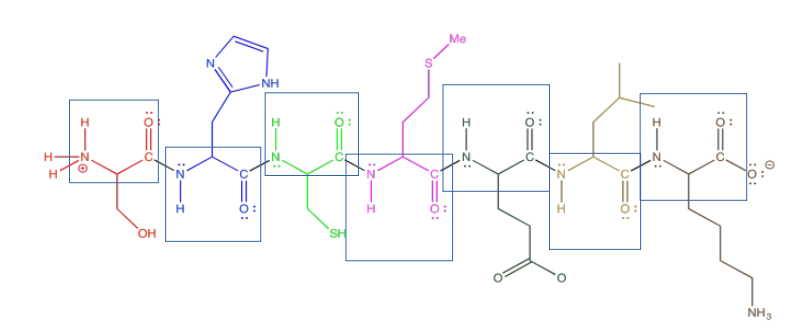
\includegraphics[width=0.5\textwidth,height=4cm]{protein.png}  % Adjust width or height as needed
  \caption{Protein}
\end{figure}





In studies that explore how genome and membrane shapes influence each other, using different modeling approaches for each component is effective. A continuum model fits well for the membrane because it captures large-scale deformations, curvature, and bending behavior without needing to simulate individual lipid molecules. This is important for understanding how the membrane flexes or reshapes in response to internal forces. On the other hand, a coarse-grained model is well-suited for the genome, as it treats the long DNA or RNA strand as a chain of simplified units, preserving essential polymer behavior like folding, looping, and confinement. This balance—continuum for the membrane and coarse-grained for the genome—allows us to efficiently simulate the mechanical interaction between the flexible genome and the deformable membrane, revealing how their shapes affect each other in confined environments.







\begin{comment}
\section*{History of Coase grained models }

Back in the 1960s and 70s—long before computational biology became mainstream—polymer scientists were already coming up with clever ways to simplify and understand how long-chain molecules behave. They built theoretical models like the freely-jointed chain, worm-like chain, and Gaussian chain, each designed to capture how flexible or stiff a polymer might be, and how it moves in space. These early ideas laid the foundation for what we now call coarse-grained simulations. Around the same time, the bead-spring model came into play — a simple but powerful way to represent a polymer as a series of connected beads linked by springs. It turned out to be incredibly useful for studying how polymers move, tangle, and interact in bulk materials — and remarkably, this same basic idea is still widely used today in modern polymer simulations.\\

Coarse-grained modeling started making an impact in protein science back in the 1970s, when researchers like Michael Levitt, Ariel Warshel, and Martin Karplus began simplifying protein structures to make them easier to study. Instead of modeling every single atom, they used a more abstract approach—sometimes representing entire amino acids as single "beads." This allowed scientists to simulate complex processes like protein folding and movement, which would have been far too computationally demanding with full atomic detail at the time. As the field evolved, so did the models. The Go model, for example, focused on capturing the folded shape of proteins in a minimalistic way, while more advanced structure-based models helped researchers understand folding pathways, domain motion, and protein aggregation. In the 2000s, the MARTINI force field took things even further, allowing proteins to be simulated in realistic environments like cell membranes and solvents. Thanks to these developments, scientists can now explore protein dynamics and interactions on scales that were once unimaginable.\\

Coarse-grained models found a natural fit in the study of lipid membranes in the early 2000s, when researchers began adapting these techniques to simulate the complex behavior of biological membranes. A major breakthrough came with the development of the MARTINI model, which represented lipids and solvents using just a few beads per molecule—typically three to four. This simplification made it possible to simulate large-scale membrane systems, including lipid bilayers, fusion events, and phase separation, all over timescales far beyond what atomistic models could handle. Scientists could now study how membrane proteins insert, move, and interact within lipid environments, as well as dynamic processes like vesicle formation, pore opening, and even viral fusion with host cells. Coarse-grained modeling also enabled the simulation of entire organelles or membrane-associated complexes that would be computationally unmanageable in full atomic detail, opening up new possibilities for understanding the structure and function of cellular membranes.\\

Coarse-grained modeling has become a vital tool for understanding how our genomes are organized and function at a large scale. Instead of trying to simulate every atom in a DNA molecule — an impossible task given that chromosomes span millions or even billions of base pairs — researchers started simplifying the problem in smart ways. Since the mid-2000s, with advances in computational power and experimental methods, researchers began modeling DNA and chromatin using coarse-grained approaches that strip away unnecessary atomic detail while keeping the essential features.

One popular method is the “bead-on-a-string” model, where each bead represents a segment of DNA or a nucleosome. These models, rooted in polymer physics, let researchers explore how DNA folds, forms loops, and compacts into the crowded space of the nucleus. Over the past decade, such models have helped understand the the folding of genome inside interpahse nulcei \cite{Lizana2024}.\\




By focusing on the big picture, coarse-grained modeling gives us a way to study the genome not just as a long string of genetic code, but as a dynamic and functional 3D structure — one that plays a critical role in how cells behave and how genes are regulated. In this research, We study how the genome and the membrane undergo shape changes and fluctuations over time.
\end{comment}




\vspace{-1em} 
\section*{Procedure} 
\subsection*{A. Kremer-Grest Model for DNA chain}

	
The Kremer-Grest (KG) model is a bead-spring type of coarse-grained model. KG model is specifically for polymers,including those relevant to chromosome structure and genome organization, and a popular way to simulate polymers in computer-based molecular dynamics. It is a specific, well-defined bead-spring model that includes Lennard-Jones (LJ) potential for excluded volume (non-bonded interactions) and FENE (Finitely Extensible Nonlinear Elastic) potential for the bonds between adjacent beads.	


\begin{figure}[!ht]
  \centering
  \fbox{\includegraphics[width=0.25\textwidth,height=4cm]{beadspring.png} }
  \caption{Bead-Spring Representation of a Polymer Chain (Kremer–Grest Model)}
\end{figure}


Instead of tracking every atom, it simplifies the system by representing each polymer chain as a string of connected beads. These beads interact with each other in two main ways: non-bonded beads repel each other using something called the Lennard-Jones (LJ) potential, which helps prevent them from overlapping, and bonded beads (those directly connected in the chain) are held together by a FENE spring, which stretches like a real polymer bond but can't break or stretch too far. To keep the system at a steady temperature—like it would be in a real fluid—a Langevin thermostat is often used, adding both friction and random kicks to the beads. The model is simple, efficient, and captures the large-scale behavior of polymers really well, which is why it's used so widely in polymer research.	



The Kremer-Grest model incorporates built-in excluded volume through the WCA potential, a modified form of the Lennard-Jones (LJ) potential that retains only the repulsive portion and removes the attractive part. This potential strongly repels beads when they come too close, preventing them from overlapping. This ensures that genome strands cannot pass through each other, similar to real physical strands that can bend and twist but cannot pass through themselves in crowded environments.

The FENE (Finitely Extensible Nonlinear Elastic) spring keeps beads connected but prevents them from stretching too far or breaking — making simulations stable even under tension or confinement.
	

Kresmer$-$grest Model is more physically realistic for polymers than a basic harmonic model and bead$-$spring model.
It prevents bond crossing by FENE and WCA and it has been extensively validated and used in thousands of studies.








\vspace{-1em} 

\subsection*{Simulation setup of Monte Carlo Simulation for a Bead-Spring Genome}
\noindent 1. System Initialization:

\setlength{\parindent}{6em} (1)Represent the genome as a chain of NN beads.

(2)Each bead has a position $\vec{r}_i = (x_i, y_i, z_i)$.

(3)Initialize positions with a non-overlapping random walk or a stretched chain.\\

\setlength{\parindent}{0pt}




2. Interaction Potential - Two energy terms used in the Coarse grain simulation:\\

\setlength{\parindent}{6em}(1)Non-Bonded Interaction-WCA potential:\\
\setlength{\parindent}{0pt}
\setlength{\parindent}{7em}For all non-bonded pairs $(i, j)$, with $|i - j| > 1$:
\setlength{\parindent}{0pt}

\begin{equation}
U_{\text{WCA}}(r) = 
\begin{cases}
4\varepsilon \left[ \left( \dfrac{\sigma}{r} \right)^{12} - \left( \dfrac{\sigma}{r} \right)^6 \right] + \varepsilon, & \text{if } r \leq 2^{1/6} \sigma \\
0, & \text{if } r > 2^{1/6} \sigma
\end{cases}
\end{equation}


\setlength{\parindent}{6em}(2)Bonded Interaction-FENE:\\
\setlength{\parindent}{0pt}
\setlength{\parindent}{8em}For each bonded pair (i,i+1)(i,i+1):

\begin{equation}
U_{\text{FENE}}(r) = -\frac{1}{2} k R_0^2 \ln \left[ 1 - \left( \frac{r}{R_0} \right)^2 \right]
\end{equation}

\setlength{\parindent}{30pt}

\begin{table}[h]
\centering
\begin{tabular}{|c|c|c|}
\hline
\textbf{Parameter} & \textbf{Meaning} & \textbf{Typical Value (KG model)} \\ \hline
$k$ & FENE spring constant & 30 \\ \hline
$R_0$ & Max bond length & 1.5 \\ \hline
$\epsilon$ & WCA strength & 1.0 \\ \hline
$\sigma$ & Bead diameter & 1.0 \\ \hline
$\delta$ & Move size & $\sim$0.1 \\ \hline
\end{tabular}
\caption{Parameters for the KG model.}
\label{tab:kg_parameters}
\end{table}



\begin{equation}
\Delta E = \Delta U_{\text{FENE}} + \Delta U_{\text{WCA}}
\end{equation}



\textbf{$\Delta E$}: This is the change in energy of the system due to the proposed move, calculated as $E_{\text{new}} - E_{\text{old}}$, where $E_{\text{new}}$ is the energy of the system after the proposed change, and $E_{\text{old}}$ is the energy before the change.


\noindent 3. Monte Carlo Move Algorithm:\\ 

\setlength{\parindent}{6em}(1)Choose a bead at random.\\
(2)Propose a small displacement:
    
\begin{equation}
    \vec{r}_i' = \vec{r}_i + \Delta \vec{r}, \quad \Delta \vec{r} \in [-\delta, \delta] 
\end{equation}

  
\setlength{\parindent}{6em}(3)Compute energy change $\Delta E$:
\setlength{\parindent}{0pt} 

\setlength{\parindent}{100pt}(i)Recalculate FENE bonds for affected neighbors.\\
(ii)Recalculate WCA interactions for all non-bonded beads within cutoff.\\
\setlength{\parindent}{0pt}


\setlength{\parindent}{6em}(4)Accept or reject using the Metropolis criterion:
\setlength{\parindent}{0pt}
\begin{equation}
P_{\text{accept}} = \min \left(1, e^{-\beta \Delta E}\right)
\end{equation}

where $\beta = \frac{1}{k_B T}$. $k_B$ is the Boltzmann constant and $T$ is the temperature of the system. $\beta$ essentially measures how sensitive the system is to energy changes at a given temperature.

\setlength{\parindent}{30pt}

This is a key expression in the Metropolis-Hastings algorithm, often used in Monte Carlo simulations, particularly in statistical physics and computational chemistry, to determine the acceptance probability of a proposed move in a system.




If $\Delta E \leq 0$ (i.e., the new state has lower or equal energy), then $e^{-\beta \Delta E} \geq 1$. The $\min$ function sets $P = 1$, meaning the move is always accepted. This makes sense because a lower-energy state is more favorable according to the Boltzmann distribution.

If $\Delta E > 0$ (i.e., the new state has higher energy), then $e^{-\beta \Delta E} < 1$, and $P = e^{-\beta \Delta E}$. The move is accepted with a probability that decreases exponentially as the energy difference $\Delta E$ increases or as the temperature $T$ decreases (since $\beta$ is inversely proportional to $T$). At low temperatures, the system is less likely to accept moves that increase energy, favoring lower-energy states.

\vspace{-1em} 
\subsection*{B. Simple liquid Models for the organelles surrounding DNA}

Simple liquid models that help understand the structure and behavior of polymer in crowded environments. Specifically, the simple liquid models referenced include Hard Sphere Model and Lennard-Jones Model. 

Hard sphere model is used to understand the behavior of particles in crowded environments, where the excluded volume effect becomes important. 

The Lennard-Jones model accounts for both attractive and repulsive forces between particles, which is important in understanding the interactions within fluids and condensed matter. It helps model the behavior of molecules, especially in non-ideal conditions like those found in crowded environments. 

\subsection*{Simulation Setup of Monte Carlo for DNA and Crowders}
\noindent 1. Define DNA Model\\
Use bead-spring polymer (FENE bonds + WCA excluded volume).\\
\noindent 2. Define Surrounding Particles (Crowders)\\
Add many free-floating particles around the DNA.\\
Interact using: WCA potential (for excluded volume) or or LJ potential\\

\noindent 3. Interaction Potentials:\\
DNA–DNA: FENE (bonded) + WCA (nonbonded)\\
DNA–Crowder: WCA or LJ\\
Crowder–Crowder: WCA or LJ\\



\noindent 4. Monte Carlo Simulation Steps:\\
(1)Initialize:\\
\setlength{\parindent}{6em} (i)Randomly place the DNA chain in the simulation box.\\
   (ii)Random positions for crowding particles (no overlaps).

\setlength{\parindent}{0em} 

\setlength{\parindent}{4em}(2)Monte Carlo Loop:\\
\setlength{\parindent}{6em}   (i)Propose random displacements for DNA beads and crowder particles.\\

(ii)For a large number of steps (e.g., $10^{5}$ or more),\\
(iii)Compute total energy:\\
\setlength{\parindent}{8em}Pick one particle (DNA bead or crowder).

Propose a small random displacement:
\begin{equation}
\mathbf{R}_{\text{new}} = \mathbf{R}_{\text{old}} + \delta
\end{equation}

\setlength{\parindent}{95pt}where \(\delta\) is random (small)
\begin{equation}
E = \sum_{\text{bonds}} U_{\mathrm{FENE}} + \sum_{\text{nonbonded}} U_{\mathrm{WCA}} 
+ \sum_{\text{DNA-crowder}} U_{\mathrm{WCA/LJ}} 
+ \sum_{\text{crowder-crowder}} U_{\mathrm{WCA/LJ}}
\end{equation}

\begin{table}[htbp]
\centering
\begin{tabular}{|c|l|}
\hline
\textbf{Parameter} & \textbf{Suggested Value} \\
\hline
$\sigma$ & Size of bead (DNA + crowder) \\
\hline
$\varepsilon$ & LJ/WCA strength (e.g., 1.0) \\
\hline
$k, R_0$ & FENE bond strength, limit \\
\hline
Number of crowders & Depends on desired volume fraction \\
\hline
\end{tabular}
\caption{Simulation parameters for the DNA-crowder system.}
\end{table}


\setlength{\parindent}{0em}
\setlength{\parindent}{6em}

(iv)Calculate energy difference:
\begin{equation}
\Delta E = E_{\text{new}} - E_{\text{old}}
\end{equation}




(v)Accept or reject moves using Metropolis criterion:
\begin{equation}
P_{\text{accept}} = \min \left(1, e^{-\beta \Delta E}\right)
\end{equation}

\setlength{\parindent}{0em}

\setlength{\parindent}{4em}
Repeat for many steps to allow the system to reach to a low-energy state with no overlaps or unphysical configurations.


\setlength{\parindent}{0em}

5. Sampling:\\
Collect statistics on DNA configurations, radius of gyration, looping, crowding effects.\\








\vspace{-1em} 
\subsection*{C. Helfrich-Canham Model for the membrane}
\setlength{\parindent}{30pt}

Membranes can be modeled at the coarse-grained level but we don't need to explicitly use a coarse-grained model. Instead, we directly use continuum models like the Helfrich-Canham model(See Figure 5). We can focus on big-scale behavior and treat the membrane as a smooth, continuous surface with properties like bending rigidity, spontaneous curvature, and surface tension. Coarse-grained models require tracking many particles, but continuum models replace them with smooth fields, making them more efficient for studying large-scale deformation








\setlength{\parindent}{30pt}
The Helfrich-Canham model, a specific type of continuum model, focuses on the membrane's curvature elasticity and bending energy\cite{Bassereau2014}.






Continuum models are a powerful framework used to describe and simulate the large-scale, smooth behavior of biological membranes (and other materials) without tracking individual atoms or molecules. Instead of focusing on discrete particles like in molecular dynamics, continuum models treat the membrane as a continuous surface or material with defined physical properties.



 

Helfrich bending energy(The simplest form)

\vspace{-1em} 


\begin{equation}
F_{\text{Helfrich}} = \int \frac{\kappa}{2} \left( 2H - C_0(\vec{r}) \right)^2 dA
\end{equation}

This is the classical Helfrich–Canham model capturing bending energy. Good for studying large-scale shape changes without worrying about connectivity changes or constraints.


\( H \) is the mean curvature\\
\( C_0(\vec{r}) \) is the spatially varying spontaneous curvature\\
\( dA \) is the surface element\\

The Helfrich–Canham model, a specific type of continuum models, focuses mainly on bending energy and curvature-driven deformations, It describes the total energy of a membrane by combining two main contributions: bending energy and surface tension energy. The bending energy reflects how much the membrane curves away from its preferred, or spontaneous, shape. Meanwhile, the surface tension energy accounts for the cost of stretching the membrane — it increases when the membrane's surface area grows. Together, these terms help explain how membranes bend, stretch, and maintain their shape in different environments.

The Helfrich–Canham model doesn't capture the details of lipid composition or molecular shape, local lipid phase transitions, specific molecular interactions, or fluctuations below the coarse-grained scale, such as nanometer-scale undulations, but it does capture large-scale bending deformations, the effects of spontaneous curvature, membrane elastic properties, shape transitions of vesicles and cells, and the response to pressure, tension, and curvature.


The total free energy of a closed lipid bilayer:\\
Continuum Form (Analytical Model):
\vspace{-1em}


\begin{align}
F_\text{full mem} = \int_S \Bigg[
&\underbrace{\frac{\kappa}{2} \left(2H - C_0(\vec{r}) \right)^2}_{(1)\ \text{spontaneous-curvature-modified bending}} 
\ + \ 
\underbrace{\bar{\kappa} K}_{(2)\ \text{Gaussian-curvature term}} 
\Bigg] dA \nonumber \\
&\quad + \ 
\underbrace{\lambda A}_{(3)\ \text{area constraint}} 
\ + \ 
\underbrace{p V}_{(4)\ \text{volume constraint}}.
\end{align}




\noindent This is a more complete energy functional for membranes.The membrane is treated as a smooth surface S.
\vspace{-2em} 
\begin{align*}
\kappa &:\ \text{bending rigidity} \\
\bar{\kappa} &:\ \text{Gaussian modulus} \\
H &:\ \text{mean curvature $= \frac{1}{2} (c_1 + c_2)$} \\
c_1,c_2 &:\ \text{principal curvatures at a point on the surface}\\
K &:\ \text{Gaussian curvature}=c_1*c_2 \\
C_0 &:\ \text{spontaneous curvature} \\
A &:\ \text{total surface area} \\
\lambda &:\ \text{Lagrange multiplier for area constraint (surface tension)} \\
P &:\ \text{Lagrange multiplier for volume constraint (pressure)}\\
V &:\ \text{Enclosed volume}\\
dA &:\ \text{Area element on the surface}\\
(2H - C_0)^2 &:\ \text{A spontaneous-curvature term for local bending preferences.}\\
\bar{\kappa} K &:\ \text{A Gaussian-curvature term for energy changes.}
\end{align*}




\vspace{-1em}

Because analytical form includes these extra factors, the full (analyzed) form describes real membranes far more accurate you’d need to estimate the mean curvature H or Gaussian curvature K at many points across the entire mesh. Even a small change in one vertex forces you to recompute normals, gradients, and curvature over dozens—or hundreds—of triangles, and then recalculate global area or volume constraints. In other words, a single vertex move would turn into a big, expensive calculation of geometry everywhere. That’s why the angle‐based form, which limits its work to just the edges touching the moved vertex, is far simpler and faster to use inside each Monte Carlo step.












It models the elastic energy of a smooth, flexible surface (like a lipid bilayer vesicle) as a function of curvature. This model alone does not specify how lipids or proteins are distributed on the surface — it just tells you what shapes minimize bending energy.








For a Monte Carlo study of a polymer confined inside a flexible membrane, the angle‐based (discrete) form is the most practical choice. The Discrete Bending Energy (Angle-based Form):
\begin{equation}
E_{\text{bend}} = \kappa \sum_{\langle i,j \rangle} \left(1 - \cos \theta_{ij} \right)
\end{equation}



\noindent is a widely used discrete approximation in simulations of triangulated membranes. While it is not directly derived from the Helfrich energy in a specific textbook, it appears in several foundational papers and review articles on triangulated surface models and coarse-grained simulations\cite{gompper1997triangulated}.

$\kappa$ is the bending rigidity,\\
$\theta_{ij}$ is the angle between adjacent triangles sharing edge $\langle i, j \rangle$.




We can distinguish between spherical and oval (ellipsoidal) shapes using the discrete form of the Helfrich energy
Discrete model is widely used in simulations (including Monte Carlo and molecular dynamics) precisely because they can capture subtle shape changes, such as the transition from a sphere to an oval.










This is a discretized approximation of the bending energy, suitable for numerical simulations Monte Carlo or molecular dynamics. It captures curvature using local triangle normals instead of differential geometry.


\begin{equation}
E_{\text{area}} = \lambda(A - A_0)^2
\end{equation}

$E_{\text{area}}$ is the area energy\\
$\lambda$ is a parameter/coefficient\\
$A$ is the current area\\
$A_0$ is the reference/target area.



Volume constraint:
\begin{equation}
E_{\text{Volume}} = \lambda(V - V_0)^2
\end{equation}

$E_{\text{Volume}}$ is the volume energy\\
$\lambda$ is a parameter/coefficient that controls the strength of the volume constraint\\
$V$ is the current volume\\
$V_0$ is the reference/target volume\\



\begin{equation}
\Delta E = (E_{\text{membrane}}^{\text{new}} + E_{\text{polymer}}^{\text{new}}) - (E_{\text{membrane}}^{\text{old}} + E_{\text{polymer}}^{\text{old}})
\end{equation}






.


Metropolis rule:
\begin{equation}
P = \min\left(1, e^{-\beta \Delta E}\right)
\end{equation}
This is a key expression in the Metropolis-Hastings algorithm, often used in Monte Carlo simulations, particularly in statistical physics and computational chemistry, to determine the acceptance probability of a proposed move in a system.


 $P$: The probability of accepting a proposed change in the system's configuration. In Monte Carlo simulations, we randomly propose changes to the system (e.g., moving a particle) and decide whether to accept or reject them based on this probability. If move is accepted then positions will be updated. If rejected then the move will be reverted.

 $e^{-\beta \Delta E}$: It is derived from the Boltzmann distribution, which describes the probability of a system being in a particular state based on its energy.

 $\beta$: This is defined as $\beta = \frac{1}{k_B T}$, where $k_B$ is the Boltzmann constant and $T$ is the temperature of the system. $\beta$ essentially measures how sensitive the system is to energy changes at a given temperature.

 $\Delta E$: This is the change in energy of the system due to the proposed move, calculated as $E_{\text{new}} - E_{\text{old}}$, where $E_{\text{new}}$ is the energy of the system after the proposed change, and $E_{\text{old}}$ is the energy before the change.


If $\Delta E \leq 0$ (i.e., the new state has lower or equal energy), then $e^{-\beta \Delta E} \geq 1$. The $\min$ function sets $P = 1$, meaning the move is always accepted. This makes sense because a lower-energy state is more favorable according to the Boltzmann distribution.

\begin{figure}[!ht]
  \centering
  \fbox{\includegraphics[width=0.25\textwidth,height=4.5cm]{fibonacci.png} }
  \caption{Sort all the vertices and make a network and identify the neighbors of A and link all the neighbors to A by Hookean spring. Introduce bending energy and curvature to vertice A.
Choose spring constant and bending energy and (may be) curvature at point A so this point will maintain concave. Meanwhile it can induce shape changes for the membrane}
\end{figure}


\subsection*{Hypothesis}

\noindent Hypothesis 1:\\
The shape of a virus forms after its genome architecture stabilizes. First, the genome reaches a steady state, and we then examine how it influences the viral membrane shape. 

\noindent Goal:\\
	(1)If the genome is 1D rod-like, the viral membrane takes an 2D elliptical shape.\\
	(2)If the genome is circular, the viral membrane forms a 2D circular shape.
	
\noindent Hyperthesis 2:\\
The genome architecture may develop after the viral membrane shape stabilizes. In this case, the membrane reaches a steady state first, and we then observe how it affects the genome’s geometry. By adjusting the length of 1D rod or the perimeter of the circle of the genome, we try to match the reference.\cite{goldsmith2003monkeypox}\\ 
\noindent Goal:\\
	(1)If the viral membrane takes an elliptical shape, the genome geometry is rod-like\cite{harish2021entomopathogenic}.	\\
	(2)If the viral membrane forms a circular shape, the genome geometry is circular.
		

	
\begin{figure}[!ht]
  \centering
  \fbox{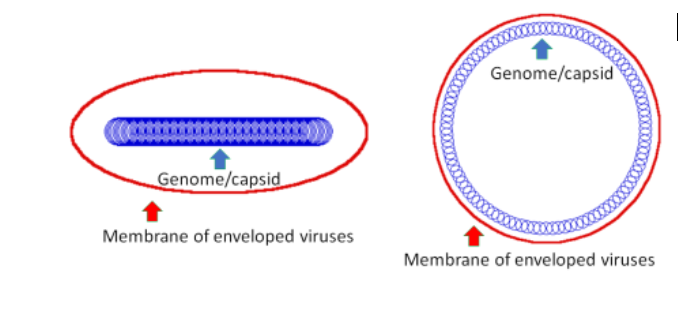
\includegraphics[width=0.5\textwidth,height=3.7cm]{monkeypox.png}}  % Adjust width or height as needed
  \caption{Preliminary 2D model studies to
investigate the effect of the geometry of a
genome on the shape of a virus. A rod-like
genome induces an elliptic shape whereas a
circular genome leads to a circular shape.}
\end{figure}
	

These viral membrane can display spherical and oval shapes, indicating different developmental stages: immature virions tend to be spherical, while mature virions adopt an oval shape. This morphological differentiation can be important for recognizing stages in the virus life cycle and understanding how these changes may affect infectivity. The transition from spherical to oval shapes may be linked to the maturation process, influencing the virus's ability to enter host cells and replicate effectively.\\

The shape of viral particles, like those seen in the Monkeypox virus, can reveal a lot about what stage they’re at in their life cycle. In the early phases, the virus forms immature virions that are usually spherical. This round shape isn’t random—it helps the virus begin assembling its genetic material and proteins in a flexible, efficient way. At this point, the virus is just starting to come together, packaging its core components. As it matures, the virus goes through structural changes that shift its shape from spherical to oval. This transformation involves the rearrangement of viral proteins, which makes the particle more stable. The oval shape not only helps the mature virion survive better outside the host but also improves its ability to attach to and enter host cells. This increased stability and better interaction with host cell receptors make the mature, oval-shaped virus more infectious and better equipped to replicate once inside a host.



We use computational methods to simulate the coupled behavior of the viral genome and membrane, allowing us to observe how changes in membrane shape influence genome configuration. Through these simulations, we can systematically vary parameters such as membrane elasticity, area and volume constraints, and genome length or stiffness to understand their roles in shaping the overall structure. This approach helps identify which physical parameters are most critical in driving morphological transitions during viral maturation. By capturing the mechanical interplay between membrane and genome, our simulations provide a powerful tool for exploring how structural constraints impact viral assembly, stability, and infectivity. Ultimately, this computational framework enhances our ability to interpret experimental observations and guides the design of more targeted experiments or antiviral strategies.\\



	
\noindent Hypothesis 3:\\
The internal pressure that builds up inside a virus’s shell during genome packaging is essential for the virus to inject its DNA or RNA into host cells. By changing the structure or mechanical properties(such as, bending rigidity ($k$)) of the capsid/membrane (such as making it weaker, stronger, or more flexible), we can control this pressure and potentially reduce the virus’s ability to infect cells.

\noindent Goal:\\
\noindent To investigate the role of internal pressure in viral genome injection and infection efficiency by:

\noindent (1) Understanding how changes in the capsid/membrane's shape and mechanical properties(bending rigidity ($k$)) affect the amount of pressure that builds up inside the virus and how easily the DNA or RNA gets out.\\

\noindent (2)Understanding which parts of the capsid/membrane are most responsible for building up and releasing pressure that helps the virus inject its DNA or RNA into host cells.\\

\begin{comment}
The genome of the Monkeypox virus is a double-stranded DNA, approximately 190 kb (kilobases) in length, which equals about 95 kbp (kilobase pairs). This genomic length corresponds to a substantial contour length of approximately 3000 nm. This indicates that the genetic material is significantly longer than the physical dimensions of the virus itself, which measures around 250 nm long. 	
\end{comment}
	
	
		





We begin by modeling the phage DNA as a fine-grained polymer, such as a worm-like chain, which accurately represents the stiffness and bending behavior of real double-stranded DNA. This model is placed within a confined volume that mimics the $60\,\text{nm} \times 150\,\text{nm}$ prolate icosahedral capsid of phage $\lambda$.
 


Next, we simulate stepwise DNA packaging by applying a force from a virtual packaging motor that mimics the biological motor’s function. At each step, a small segment of DNA is inserted into the capsid, and we calculate the energy required to overcome internal forces such as electrostatic repulsion and bending stress. This allows us to track the buildup of internal pressure as the capsid fills, which can then be directly compared to experimentally measured force-extension (packing) curves from optical tweezer studies.

Once the genome is fully packaged, we simulate ejection dynamics by triggering a release mechanism, such as opening a virtual portal in the capsid. The DNA is then allowed to eject, and we record the ejection speed, force, and time as the internal pressure drives the genome out. These simulation results can be compared to experimental data from ejection assays and osmotic suppression experiments, where external osmotic agents slow or block ejection and allow researchers to measure the pressure driving it.


By tuning simulation parameters (e.g., DNA stiffness, packing force, ionic strength) and validating against high-quality experimental datasets from phage $\lambda$, we ensure that our model reproduces the biological and physical behavior observed in the lab. In bacteriophages, the DNA experiences strong forces—up to around 60 picoNewtons—during the packaging and ejection process. These forces mainly come from the bending stiffness of the DNA and the repulsion between tightly packed strands. Experiments using osmotic suppression have shown that it's possible to stop DNA ejection by applying external PEG solutions that create about 20 to 40 atmospheres of pressure\cite{Grayson2006}.







Simulating realistic physical conditions, since many experiments happen at constant pressure (example:1 atm) and temperature  (example: 298 K).

\noindent NPT Ensemble (Isothermal–Isobaric Ensemble)

NPT stands for:

    N = Number of particles (constant)

    P = Pressure (constant)

    T = Temperature (constant)
    
    Under NPT conditions, the system’s pressure is controlled, allowing the volume to change naturally over time. In one approach, the membrane is initialized with a fixed oval or ellipsoidal shape, defined by the input parameters a, b, and c, which represent the lengths along its three principal axes. These parameters remain constant during the simulation, so the membrane maintains its overall shape while still allowing local fluctuations and interactions with the genome inside.

In another approach, the parameters a, b, and c are allowed to fluctuate during the simulation. This means the membrane can expand, shrink, or reshape dynamically in response to internal forces exerted by the genome. Such flexibility promotes more realistic interactions between the genome and the membrane — for example, the genome may push outward and deform the membrane, while changes in membrane tension or curvature can influence how the genome is organized. Using NPT conditions in this way provides a natural and dynamic view of the interplay between membranes and genomes in biological systems.

\noindent NVT Ensemble (Canonical Ensemble)

NVT stands for:

    N = Number of particles (constant)

    V = Volume (constant)

    T = Temperature (constant)

Under NVT conditions, the volume of the system is fixed, meaning the membrane is constrained and cannot expand or contract. In one approach, the membrane is initialized with an oval or ellipsoidal shape, defined by input parameters a, b, and c, representing the lengths along its three principal axes. These parameters remain constant throughout the simulation, so the membrane keeps its shape even as the genome inside moves or grows. Because the membrane cannot adapt naturally to changes, any pressure exerted by the genome builds up inside, sometimes leading to artificial forces that would not normally appear in a flexible system.

In another approach, even though the overall volume remains fixed under NVT, small local fluctuations in the shape of the membrane are allowed while still keeping a, b, and c centered around their initial values. In this case, the membrane can slightly deform in response to internal forces from the genome without changing its total volume. While the confinement effect is still strong, allowing limited local fluctuations provides a somewhat more realistic interaction between the genome and the membrane. Studying the membrane–genome relationship in either method under NVT is useful for early-stage stabilization or when specifically exploring how genomes behave in confined, rigid environments.

\subsection*{Timeline}
Months 0-3: Fine-tune the continuum membrane model.\\
Months 4-6: Investigate competition among different membrane shapes.\\
Months 7-9: Study chain model and crowding effect\\
Months 10-12:Expand the developed models from 2D to 3D.



\end{flushleft}


\newpage



\bibliographystyle{unsrt}
\bibliography {references}  

\end{document}




